\documentclass[11pt]{article}
\usepackage[a4paper, total={6in, 8in}]{geometry}
\usepackage{float}
\usepackage{multirow}    % to add multirow cells in tables
\usepackage{indentfirst} % to automatically indent the first paragraph of each section
\usepackage{amsmath}     % math packages
\usepackage{mathtools}
\usepackage{amssymb}
\usepackage{graphicx}    % Required for inserting images
\usepackage{fontenc}
\usepackage[colorlinks=true,linkcolor=blue,citecolor=blue, urlcolor=blue]{hyperref} % for hyperlinks
\usepackage{subcaption}  % to add subcaptions within single floating environments
\usepackage{placeins}    % to control the position of floating environments
\usepackage[numbers]{natbib}  % for correct formatting of bibliography
\usepackage{import}
\usepackage[utf8]{inputenc}
\usepackage{tikz}
\usepackage{tikz-cd}
\usepackage{pgfplots}
\pgfplotsset{compat=1.14}
\bibliographystyle{abbrvnat}
\usepackage{siunitx} % for correct formatting of units
\sisetup{separate-uncertainty=true}
\providecommand{\mathdefault}[1]{\mathrm{#1}}
\DeclareMathOperator{\arctanh}{arctanh}
% Define atomic mass unit (u)
\sisetup{per-mode=symbol}
\DeclareSIUnit\atomicmassunit{u}

\title{Auswertung von Versuch FP43: Raman-Spektroskopie}
\author{Coc, Q'inich and Huth, Paris}
\date{January 2025}

\begin{document}
\maketitle

\section{Charakterisierung des Raman-Kantenfilters}
Im ersten Teil des Versuchs messen wir die Abhängigkeit der Photodiodenspannung vom Einfallswinkel. Die Messreihe wird in Fig. \ref{fig:justierung} dargestellt. Zusätzlich wird ein linearer Fit an den Flanken der Kurve angepasst.

\begin{figure}[htbp]
	\centering
   \resizebox{.8\textwidth}{!}{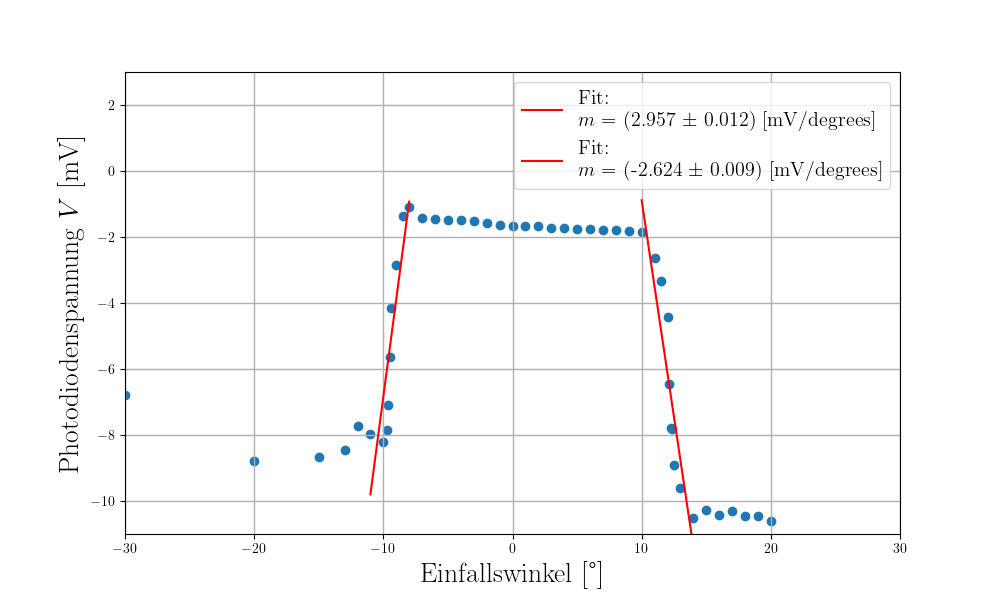
\includegraphics{Justierung.png}}
   \caption{Gemessene Abhängigkeit der Photodiodenspannung vom Einfallswinkel (blaue Punkte) zusammen mit dem linearen Fit der Flanken der Kurve (rote Linien).}
   \label{fig:justierung}
\end{figure}

Während der Durchführung dieses Versuchsteils bemerkten wir, dass der Laser nicht stabil war, da die Intensität des Lasers signifikant abnahm, bis keine Messungen mehr durchgeführt werden konnten. Unser Betreuer konnte das Problem erfolgreich beheben.

Um die Cut-on-Winkel aus diesem Diagramm zu ermitteln, passen wir einen weiteren Fit an das Plateau der Kurve an. Zunächst berechnen wir die Schnittstellen der Flankenfits mit diesem letzten Fit. Wir schätzen folgende Cut-on-Winkel:
$$\vartheta_1 =  \SI{-8.18\pm 0.17}{\degree}$$ 
$$\vartheta_2 =  \SI{10.36\pm 0.21}{\degree}$$ 

Im zweiten Schritt messen wir die Abhängigkeit der Zählrate von der angelegten Beschleunigungsspannung $U_B$, um die sogenannte PMT-Kennlinie darzustellen. Während der Durchführung dieses zweiten Versuchsteils traten erneut Fehler bei den Messungen auf, die aufgrund der Instabilität des Lasers verursacht wurden. Das fehlerhafte Verhalten des Lasers ist deutlich in Fig. \ref{fig:fehler} zu erkennen. In diesem Diagramm sind unsere Messungen zu sehen, die signifikant von den Erwartungen abweichen. Die Probleme mit dem Laser waren zu komplex, und das Gerät konnte nicht schnell genug repariert werden, um weitere Messungen durchzuführen. Aus diesem Grund erhielten wir alte Messwerte von unserem Betreuer, um die Auswertung des Versuchs durchzuführen.

\begin{figure}[htbp]
    \centering
    % First row
    \begin{subfigure}{0.45\textwidth}
        \centering
        \resizebox{1.0\textwidth}{!}{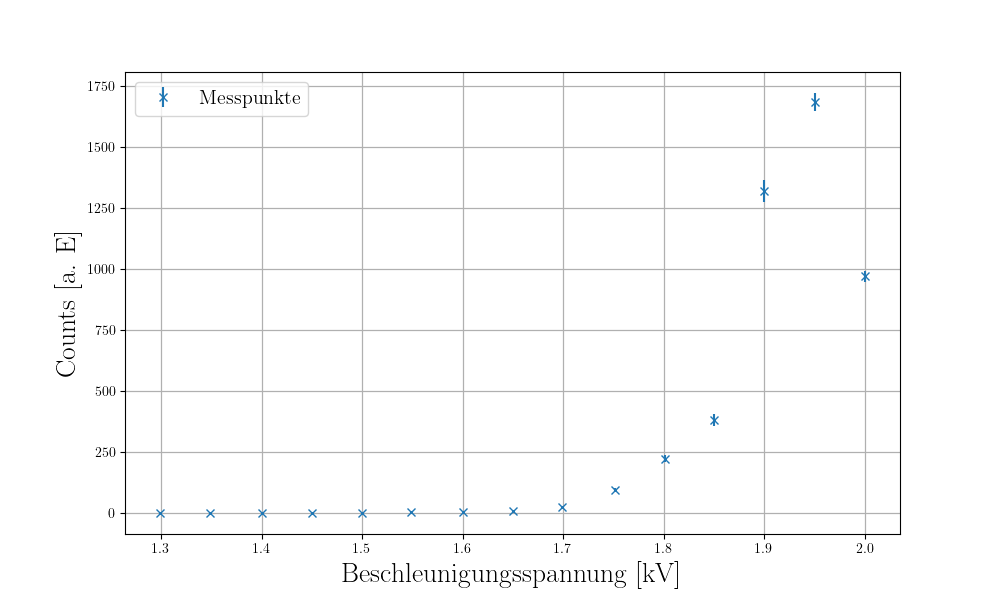
\includegraphics{PMT_Kennlinie_fail.png}}
        \caption{}
        \label{fig:fehler}
    \end{subfigure}
    \hfill
    \begin{subfigure}{0.45\textwidth}
        \centering
        \resizebox{1.0\textwidth}{!}{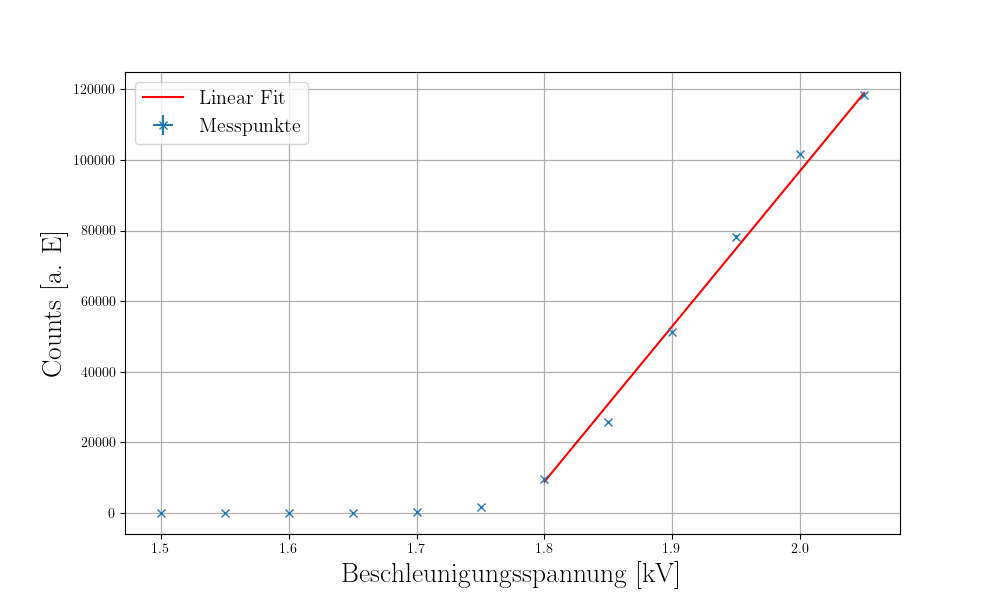
\includegraphics{PMT_Kennlinie.png}}
        \caption{}
        \label{fig:gegeben}
    \end{subfigure}
    % Second row
    \caption{PMT-Kennlinie. Abhängigkeit der Zählrate von der angelegten Beschleunigungsspannung. a) Messreihe mit fehlerhaftem Laser. b) Messreihe mit funktionsfähigem Laser mit linearem Fit (alte Messwerte vom Betreuer erhalten).}
    \label{fig:PMT_Kennlinie}
\end{figure}

In Fig. \ref{fig:gegeben} wird die PMT-Kennlinie des verwendeten Raman-Filters dargestellt . Aus diesem Diagramm können wir erkennen, dass im Bereich von \num{1.8} bis \SI{2.0}{\kilo\volt} die Zählrate ein fast lineares Verhältnis zu $U_B$ zeigt. 
% todo nicht linear
Um sinnvolle Messungen durchzuführen, muss das Signal-zu-Rausch-Verhältnis maximiert werden. Daher können wir eine Spannung von $U_B =$ \SI{2.0}{\kilo\volt} als eine gute Wahl angeben.

\section{Raman-Spektrum}
In diesem Versuchsteil untersuchen wir das Raman-Spektrum von den zwei Kernspinisomeren von Protium und das Spekturm von Deuterium, Sauerstoff und Stickstoff. Zu jeder Messreihe gehört ein gemessenes Untergrundspektrum, das vom Spektrum abgezogen werden muss, um die Zählrate der ramangestreuten Photonen zu isolieren.

\subsection{Rotationsspektrum von Deuterium}
Aus dem gemessenen Deuterium-Spektrum, Fig. \ref{fig:Deuterium}, können wir vier Raman-Linien beobachten. Um die gefundenen Linien benennen zu können, müssen wir zunächst die erwarteten Wellenzahlen der Linien bestimmen.

Die Bestimmung der erwarteten Position der Raman-Linien wird mit den Literaturwerten der Masse von Deuterium und dem Atomabstand eines Deuteriummoleküls $D_2$ durchgeführt:
$$m_{D} =\SI{2.01588}{\atomicmassunit}$$
$$r_{D_2} = \SI{74}{\pm}.$$
Diese Werte setzen wir in die Gleichung
\begin{equation}
\label{eq:Rot_const}
B = \frac{h}{8\pi^2 c \mu r^2}
\end{equation}
ein, um die erwartete Rotationskonstante zu bestimmen. Hierbei entspricht $h$ der Planck-Konstante, $c$ der Lichtgeschwindigkeit und $\mu$ der reduzierten Masse:
\begin{equation}
\label{eq:redu_mass}
\mu = \dfrac{m_1 \cdot m_2}{m_1 + m_2}.
\end{equation}
Da wir mit homogenen Molekülen arbeiten, gilt $m_1 = m_2$, und Gl. \ref{eq:redu_mass} vereinfacht sich zu:
\begin{equation}
\mu = \dfrac{1}{2} m.
\end{equation}
Wir finden: 
$$B_{lit}^{D_2} = \SI{30.57}{cm^{-1}}.$$
Die Wellenzahl der Rotationsanregungen wird durch
\begin{equation}
\label{eq:nu_rot,j} 
\bar{\nu}_{rot,J} = B(4J+6)
\end{equation}
gegeben. Die Wellenzahl der Raman-Linie kann durch
\begin{equation}
\bar{\nu}_{J\to J+2} = \bar{\nu}_{Laser} \pm \bar{\nu}_{rot,J}
\end{equation}
ermittelt werden. In unserem Experiment gilt:
$$\bar{\nu}_{Laser} = \SI{18777.58}{\centi\meter^{-1}}$$

Um die Position der gemessenen Raman-Linien quantitativ zu betrachten, passen wir eine Voigt-Verteilung an die einzelnen erkennbaren Peaks an, und als Fit-Funktion wird die Summe der einzelnen angepassten Voigt-Profile verwendet. Die Voigt-Verteilung ist durch die Faltung einer Gauß- und einer Breit-Wigner-Verteilung definiert. Die Messwerte und die Fit-Funktion werden in Fig. \ref{fig:Deuterium} dargestellt. 

Durch Vergleich der gemessenen und erwarteten Position der Linien können wir die gemessenen Raman-Linien als die ersten vier Rotationsanregungen erkennen. Die gefundenen und erwarteten Werte werden in Tab. \ref{tab:D2} zusammengefasst und verglichen.

\begin{figure}[htbp]
	\centering
   \resizebox{1.0\textwidth}{!}{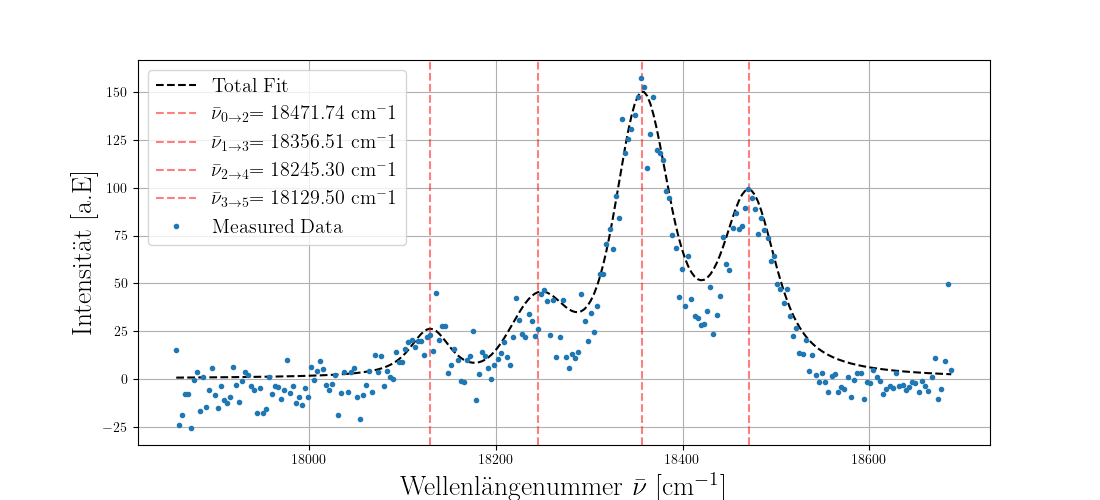
\includegraphics{D2_spektrum}}
   \caption{\small Raman-Spektrum von Deuterium. Gemessenes Spektrum einer Deuterium-Probe nach Untergrundabzug (blaue Punkte) mit Fit-Funktion, die aus der Summe der einzelnen Voigt-Fits besteht (schwarze Linie). Die gefundenen Raman-Linien sind durch gestrichelte rote Linien markiert.}
   \label{fig:Deuterium}
\end{figure}

\begin{table}[!htbp]
 \begin{center}
  \caption{\small Wellenzahl der Raman-Linien von $D_2$. Vergleich von erwarteten und gemessenen Werten.}
   \renewcommand{\arraystretch}{1.3} % Adjust 1.5 as needed
  \label{tab:D2}
  \begin{tabular}{|c|c|c|c|}
  \hline
\multirow{2}{*}{$J$}& \multicolumn{2}{c|}{$\bar{\nu}_{J\to J+2}$ [$\unit{cm^{-1}}$]} &  \multirow{2}{*}{ Abweichung $\sigma$} \\ \cline{2-3} % Horizontal line under the multicolumn
 					 & gemessen & erwartet &    			\\ 
  \hline
	\hline 
0 & $\num{18471.7\pm 1.1}$	& 18507.17	& 33.4 \\
1 & $\num{18356.5	\pm 0.9}$	& 18385.88	& 31.3 \\
2 & $\num{18245\pm 3}$	& 18263.60	& 6.5	 \\
3 & $\num{18129\pm 4}$	& 18141.32	& 3.22 \\
	\hline
  \end{tabular}
  \renewcommand{\arraystretch}{1} 

 \end{center}
\end{table}

Durch Bestimmung des Abstands zwischen den Peaks können wir die Rotationskonstante von Deuterium bestimmen, indem wir Gl. \ref{eq:nu_rot,j} verwenden. Auf diese Weise können wir drei Werte für $B$ berechnen. Als Endergebnis werden der Mittelwert und die zugehörige Standardabweichung verwendet: 
$$B_{exp}^{D_2} = \SI{28.5\pm 0.5}{cm^{-1}}.$$
Wir beobachten eine signifikante Abweichung vom erwarteten Wert:
$$\sigma_{B^D_2} = 4.01$$ 
 
Durch Umstellen von Gl. \ref{eq:redu_mass} können wir die reduzierte Masse $\mu$ abschätzen:
$$\mu_{exp}^{D_2} = \SI{1.079\pm 0.019}{\atomicmassunit}.$$
Dieser Wert zeigt ebenfalls eine signifikante Abweichung vom erwarteten Wert $\mu_{lit} = \dfrac{1}{2}m_D$:
$$\sigma_{\mu^D_2} = 3.74.$$
Die großen Abweichungen werden später ausführlich besprochen.

\subsection{Rotationsspektrum von normal- und para-Wasserstoff}
Zunächst führen wir eine ähnliche Analyse wie bei Deuterium mit dem gemessenen Spektrum von normal- und para-Wasserstoff durch.

Für die Bestimmung der erwarteten Rotationskonstante und Wellenzahl der Raman-Linien verwenden wir folgende Werte für den Abstand von $H_2$ und die Masse von $H$:

$$m_{H} =\SI{1.00794}{\atomicmassunit}$$
$$r_{H_2} = \SI{74}{\pm}.$$
Durch Einsetzen dieser Werte in Gl. \ref{eq:Rot_const} finden wir:
$$B_{lit}^{H_2} = \SI{61.0841}{cm^{-1}} $$

Analog zum letzten Abschnitt passen wir eine Voigt-Verteilung an jeden erkennbaren Peak an und bilden die Fit-Funktion aus der Summe der einzelnen Voigt-Fits. Als Wellenzahl wird die Position des Maximums der Verteilung und der zugehörige Fehler angegeben. Das gemessene Spektrum von normalem $H_2$ zusammen mit der Fit-Funktion wird in Fig. \ref{fig:normal_H2} dargestellt. Das Spektrum der para-$H_2$-Probe wird in Fig. \ref{fig:para_H2} gezeigt. Mithilfe dieses Diagramms stellen wir fest, dass die Untergrundmessung der para-$H_2$-Probe nicht erfolgreich war, da nach dem Untergrundabzug eine Verschiebung des Spektrums um ca. 43 a.E. in der y-Achse beobachtet wird.

Durch Vergleich der erwarteten und gemessenen Wellenzahl der Raman-Spektren von Wasserstoff können wir die gefundenen Peaks als die ersten Rotationsanregungen erkennen. Die gemessenen und erwarteten Wellenzahlen der Raman-Linien werden in Tab. \ref{tab:H2} zusammengefasst und verglichen. Zusätzlich wird die Intensität der Raman-Linien in derselben Tabelle zusammengefasst, um die Reinheit des para-Wasserstoffs abzuschätzen.

\begin{figure}[htbp]
	\centering
   \resizebox{1.0\textwidth}{!}{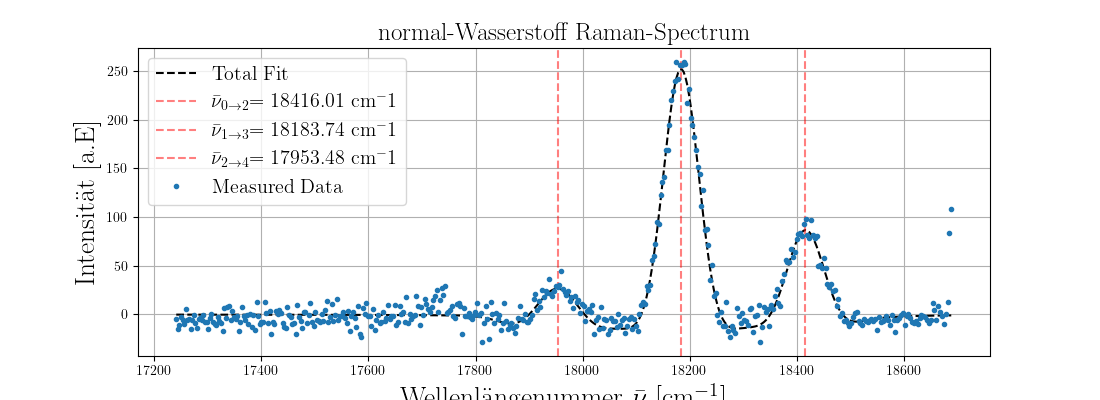
\includegraphics{H2_spektrum.png}}
   \caption{\small Raman-Spektrum von normal-Wasserstoff. Gemessenes Spektrum einer normalen Wasserstoff-Probe nach Untergrundabzug (blaue Punkte) mit Fit-Funktion (schwarze Linie). Die gefundenen Raman-Linien sind durch gestrichelte rote Linien markiert.}
   \label{fig:normal_H2}
\end{figure}

\begin{figure}[htbp]
	\centering
   \resizebox{1.0\textwidth}{!}{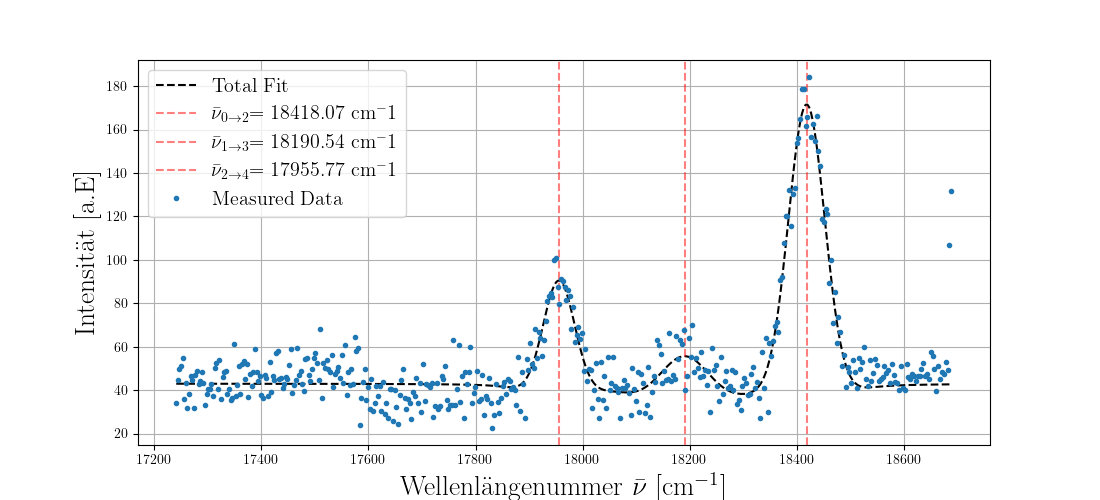
\includegraphics{paraH2_spektrum.png}}
   \caption{\small Raman-Spektrum von para-Wasserstoff. Gemessenes Spektrum einer normalen Wasserstoff-Probe nach Untergrundabzug (blaue Punkte) mit Fit-Funktion (schwarze Linie). Die gefundenen Raman-Linien sind durch gestrichelte rote Linien markiert.}
   \label{fig:para_H2}
\end{figure}

Wie erwartet können wir sehen, dass die Raman-Linien der ungeraden Vibrationsquanten im para-$H_2$-Spektrum unterdrückt werden, Fig. \ref{fig:para_H2}, da diese zu ortho-Wasserstoff gehören. Wir erinnern uns, dass die beiden Wasserstoffisomeren Spin 0 (para) und 1 (ortho) besitzen und daher nur gerade (para) oder ungerade (ortho) Zustände zulassen, aber nicht beide. Die kleine, aber endliche Intensität der zweiten Rotationsanregung, $I_{\nu  = 1 \to 3}$, zeigt, dass die para-Wasserstoff-Probe noch eine endliche Anzahl an ortho-$H_2$ enthält. Durch Berechnung des Verhältnisses zwischen der Intensität der ersten $I_{\nu  = 0 \to 2}$ und der zweiten $I_{\nu  = 1 \to 3}$ Raman-Linie können wir feststellen, dass die para-$H_2$-Probe aus 1 Teil ortho- und 25 Teilen para-Wasserstoff besteht (1:25). Daher besteht die Probe zu ca. $96.2\%$ aus para-Wasserstoff, und die Reinheit kann als hoch beurteilt werden. Wird das Verhältnis der beiden Intensitäten mit den Fitparametern des normalen Wasserstoffs berechnet

\begin{equation}
	\frac{g_\text{normal}}{g_\text{para}}=3\cdot\frac{I_\text{normal}^0}{I_\text{normal}^1}\cdot\frac{I_\text{para}^0}{I_\text{para}^1},
\end{equation}

so finden wir, dass die Probe ein Verhältnis von 3:1 beschreibt, was mit der Literatur übereinstimmt.

\begin{table}[!htbp]
 \begin{center}
  \caption{\small Wellenzahl der Raman-Linien von $H_2$. Vergleich von erwarteten und gemessenen Werten einer para- und normalen Wasserstoffprobe.}
  \label{tab:H2}
  % Increase the row height
  \renewcommand{\arraystretch}{1.3} % Adjust 1.5 as needed
  \begin{tabular}{|c|c|c|c|c|c|c|c|}
  \hline
\multirow{2}{*}{$J$}&\multicolumn{2}{c|}{Intensität [a.E]}& \multicolumn{3}{c|}{$\bar{\nu}_{J\to J+2}$ [$\unit{cm^{-1}}$]} & \multicolumn{2}{c|}{ Abweichung $\sigma$} \\ \cline{2-8} % Horizontal line under the multicolumn
 					 &$H_2^{norm.}$	&	$H_2^{para}$ & gem. $H_2^{norm.}$ & gem. $H_2^{para}$& erwartet &  $H_2^{norm.}$	&	$H_2^{para}$\\ 
  \hline
	\hline 
0 &	$\num{5211\pm450}$ 	&	$\num{10035\pm577}$	&	$\num{18416	\pm 1}$	& $\num{18418.1\pm 1}$	& 18325.08	& 91.8	& 116.12 \\ 
1 & 	$\num{16699\pm395}$	&	$\num{448\pm348}$	&	$\num{18183.7\pm0.4}$& $\num{18191\pm6}$	& 18080.75	& 279.12	& 18.78 \\ 
3 &	$\num{627\pm237}$	&	$\num{2926\pm333}$	&	$\num{17953\pm2}$	& $\num{17956\pm2}$	& 17836.41	& 53.59	& 76.24\\ 
	\hline
  \end{tabular}
  % Reset the row height to default
  \renewcommand{\arraystretch}{1}
 \end{center}
\end{table}

Aus der Tabelle können wir ersehen, dass erneut signifikante Abweichungen zwischen den erwarteten und gemessenen Werten bei beiden Messreihen, d.h. normalem und para-$H_2$, auftreten.

Durch Bestimmung des Abstands zwischen den gemessenen Raman-Linien lassen sich zwei Werte für die Rotationskonstante und zwei Werte für die reduzierte Masse berechnen, die wir in Tab. \ref{tab:H2_B_mu} zusammenfassen und vergleichen.

\begin{table}[!htbp]
 \begin{center}
  \caption{\small Wellenzahl der Raman-Linien von $H_2$. Vergleich von erwarteten und gemessenen Werten einer para- und normalen Wasserstoffprobe.}
  \label{tab:H2_B_mu}
  % Increase the row height
  \renewcommand{\arraystretch}{1.3} % Adjust 1.5 as needed
  \begin{tabular}{|c|c|c|c|c|c|}
  \hline

\multirow{2}{*}{Größe}&\multicolumn{3}{c|}{Wert}& \multicolumn{2}{c|}{ Abweichung $\sigma$} \\ \cline{2-6} % Horizontal line under the multicolumn
 					 &$H_2^{norm.}$	&	$H_2^{para}$ &  $H_2^{lit}$ &  $H_2^{norm.}$	&	$H_2^{para}$\\ 
  \hline
	\hline 
B [$\unit{cm^{-1}}$] & $\num{57.8\pm0.3}$ & $\num{57.8\pm0.9}$ & 61.0841 & 13.03 & 3.64 \\
$\mu$ [$\unit{\atomicmassunit}$] & $\num{0.532\pm0.002}$& $\num{0.5\pm0.3}$&0.5004 &15.8 & 0.001\\
	\hline
  \end{tabular}
  % Reset the row height to default
  \renewcommand{\arraystretch}{1}
 \end{center}
\end{table}

Aus Tab. \ref{tab:H2_B_mu} lässt sich der Einfluss der fehlerhaften Untergrundmessung für para-$H_2$ erkennen. Die Verschiebung in der y-Achse hat die Genauigkeit der Fitparameter stark reduziert, im Vergleich zum normalen $H_2$. Für die Fits wurde versucht, die Verschiebung in y-Richtung zu berücksichtigen, dennoch bleibt die große Unsicherheit der Fitparameter bestehen. Aus diesem Grund sind die Abweichungen kleiner als beim normalen $H_2$, obwohl die Werte nicht signifikant näher am Literaturwert liegen. Die beobachteten signifikanten Abweichungen werden später in der Diskussion behandelt.

\subsubsection{Breite der Peaks}
Die gemessenen Spektren von Deuterium, Fig. \ref{fig:Deuterium}, und beiden Wasserstoffproben, Fig. \ref{fig:normal_H2}-\ref{fig:para_H2}, zeigen eine Linienverbreiterung, d.h. die Vergrößerung der Linienbreite unserer Raman-Linien. Diese Verbreiterung kann durch verschiedene physikalische Phänomene verursacht werden.

Eine der Quellen dieser Verbreiterung ist die sogenannte Dopplerverbreiterung. Dieses Phänomen beschreibt die Verbreiterung der Spektrallinien zu einem Band aufgrund des Doppler-Effekts, der durch die thermische Bewegung der Moleküle in der Probe verursacht wird. Dieser Effekt auf die Wellenlänge kann mithilfe der Maxwell-Boltzmann-Verteilung quantifiziert werden:
\begin{equation}
\label{eq:dopp_breite}
\delta \lambda = \dfrac{\lambda}{c} \sqrt{\dfrac{8k_B T \ln 2}{m_{M}}}. 
\end{equation}
Wobei $k_B$ die Boltzmann-Konstante, $T$ die Temperatur, $\lambda$ die Frequenz der Spektrallinien und $m_{M}$ die Masse des Moleküls ist. Um den Einfluss dieses Effekts auf die Verbreiterung quantitativ zu betrachten, berechnen wir die erwartete Breite der ersten Spektrallinie für Deuterium, d.h. die $0\to 2$ Rotationsanregung, und vergleichen sie mit unseren Fitparametern. Die Temperatur des Raums wurde leider während des Versuchs nicht aufgezeichnet, aber wir schätzen sie auf $T = \SI{16}{\degree} = \SI{289.15}{K}$, und die Masse des Moleküls wird durch das Doppelte der Masse von Deuterium gegeben.

Die gemessene Breite der Raman-Linie wurde als
$$\delta \lambda = \SI{0.885 \pm 0.005}{\nano\meter}$$
bestimmt. Durch Verwendung von Gl. \ref{eq:dopp_breite} schätzen wir
$$\delta \lambda =  \SI{3.284\pm 0.005}{\pico\meter}$$
ab. Diese schnelle Abschätzung zeigt, dass, obwohl die Dopplerverbreiterung zur Breite der Spektrallinien beiträgt, dieses Phänomen allein die gemessene Breite der Rotations-Raman-Linien nicht erklären kann.

Wir vermuten, dass andere Verbreiterungsquellen wie die Energie-Zeit-Unschärferelation und die Auflösung unseres Detektors zur gemessenen Breite beitragen. Leider sind weder die Lebensdauer des virtuellen Zustands noch das Auflösungsvermögen unseres Detektors bekannt, um diese weiteren Phänomene qualitativ abschätzen zu können.

\subsection{Vibrationsanregung von Sauerstoff und Stickstoff}
In diesem letzten Abschnitt betrachten wir das Vibrations-Raman-Spektrum von Stickstoff und Sauerstoff. Aufgrund der höheren reduzierten Masse und des größeren Atomabstands beider Moleküle ist die Rotationskonstante deutlich kleiner als die Rotationskonstante von Wasserstoff, und die Auflösung unseres Versuchsaufbaus ist nicht hoch genug, um die Rotationsstruktur aufzulösen. Trotzdem können wir, da die Vibrationsanregungen eine höhere Energie besitzen, die erste Schwingungsanregung auflösen und messen.

\begin{figure}[htbp]
	\centering
   \resizebox{1.0\textwidth}{!}{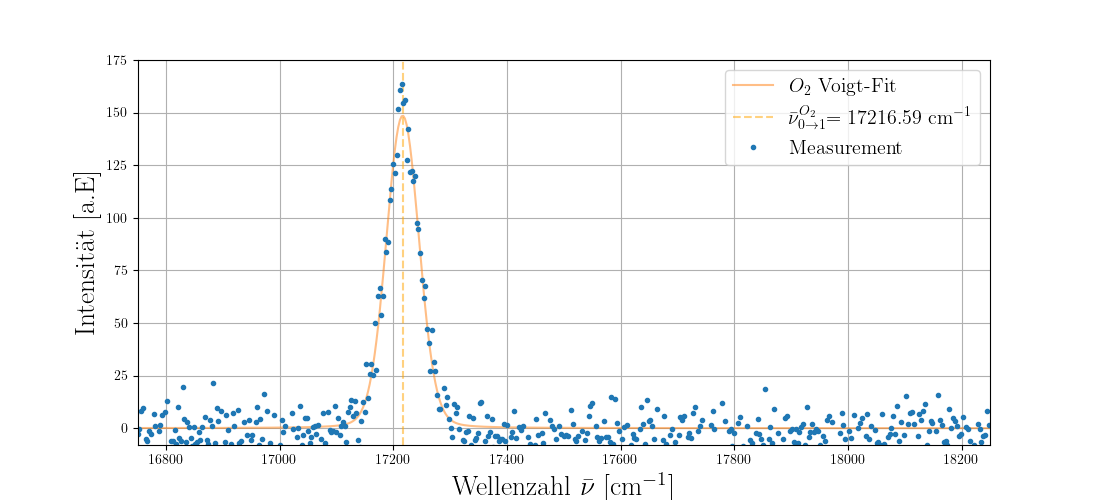
\includegraphics{02_spektrum.png}}
   \caption{\small Raman-Spektrum von Sauerstoff. Gemessenes Spektrum einer normalen Wasserstoff-Probe nach Untergrundabzug (blaue Punkte) mit Fit-Funktion (orange Linie). Die gefundene Raman-Linie ist durch eine gestrichelte orange Linie markiert.}
   \label{fig:O2}
\end{figure}

\begin{figure}[htbp]
	\centering
   \resizebox{1.0\textwidth}{!}{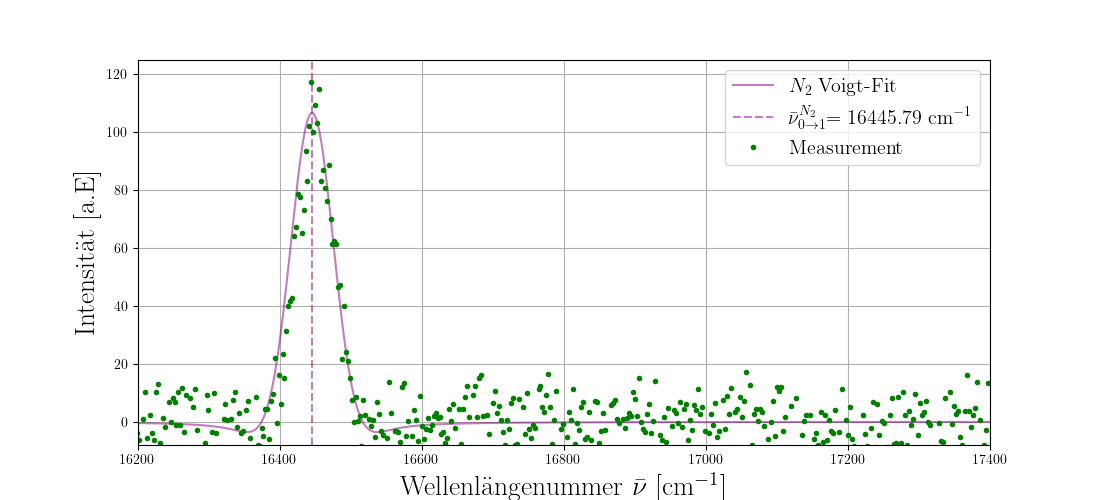
\includegraphics{N2_spektrum.png}}
   \caption{\small Raman-Spektrum von Stickstoff. Gemessenes Spektrum einer normalen Wasserstoff-Probe nach Untergrundabzug (grüne Punkte) mit Fit-Funktion (lila Linie). Die gefundene Raman-Linie ist durch eine gestrichelte lila Linie markiert.}
   \label{fig:N2}
\end{figure}

Analog zu den vorherigen Versuchsteilen passen wir ein Voigt-Profil an die Peaks unserer Messungen an. Die Messdaten und die Fit-Funktion werden in Fig. \ref{fig:O2} und \ref{fig:N2} dargestellt. Aus den Fitparametern können wir die Wellenzahl unserer gemessenen Raman-Linien ablesen:

$$\bar{\nu}^{O_2}_{exp} = \SI{17216.6\pm 0.5}{cm^{-1}}$$
$$\bar{\nu}^{N_2}_{exp} = \SI{16446\pm 6}{cm^{-1}}$$

und sie in die Gleichung
\begin{equation}
E_{vib} = hc\bar{\nu}_{Laser} - hc\bar{\nu}_{Fit}
\end{equation}
einsetzen, um die Schwingungsübergangsenergie zu bestimmen.

In der Literatur [W. Hack, Molekülephysik und Quantenchemie] finden wir folgende Werte für die Raman-Linien:
$$\bar{\nu}^{O_2}_{lit} = \SI{17135.29}{cm^{-1}}$$
$$\bar{\nu}^{N_2}_{lit} = \SI{16360.89}{cm^{-1}}$$

Die berechneten und gemessenen Werte werden in Tab. \ref{tab:N_O} zusammengefasst. Zusätzlich wird die Abweichung zwischen beiden Werten eingetragen. Hier können wir sehen, dass die gemessenen Werte doppelt so groß sind wie die erwarteten, was einen übertrieben großen $\sigma$-Wert erzeugt. Leider können wir keinen Fehler in unseren Berechnungen finden, der diese Differenz verursachen würde. Mögliche Fehlerquellen werden später diskutiert.

\begin{table}[!htbp]
 \begin{center}
  \caption{ \small Schwingungsübergangsenergie von Sauerstoff und Stickstoff.}
  \label{tab:N_O}
  \renewcommand{\arraystretch}{1.3}
  \begin{tabular}{|c|c|c|c|}
  \hline

\multirow{2}{*}{Molekül}& \multicolumn{2}{c|}{$E_{vib}$ [$\unit{\milli\electronvolt}$]} &  \multirow{2}{*}{ Abweichung $\sigma$} \\ \cline{2-3} % Horizontal line under the multicolumn
 					 & gemessen & erwartet &    			\\
  \hline
  \hline
  $O_2$	&	$\num{182.88 \pm 0.07}$	&	$\num{192.95}$ &	1311\\
  $N_2$	&	$\num{278.4 \pm 0.5}$	&	$\num{288.96}$&	261\\ 
  \hline
  \end{tabular}
  \renewcommand{\arraystretch}{1}
 \end{center}
\end{table}

\section{Zusammenfassung und Diskussion}
In diesem Versuch haben wir Raman-Spektroskopie verwendet, um die Rotations- und Schwingungseingenschaften verschiedener Moleküle zu untersucht.

Der Versuch begann mit der Charakterisierung des Raman-Kantenfilters, bei dem die Abhängigkeit der Photodiodenspannung vom Einfallswinkel gemessen wurde. Dabei wurden die Cut-on-Winkel von $\vartheta_1 = \left(-8.18\pm 0.17\right)^\circ$ und $\vartheta_2 =\left(10.36\pm 0.21\right)^\circ$ bestimmt. 

Im nächsten Schritt wurde die PMT-Kennlinie untersucht, um die Abhängigkeit der Zählrate von der angelegten Beschleunigungsspannung $U_B$ zu bestimmen. Hier zeigte sich, dass im Bereich von $1.8-2.0$ kV die Zählrate linear von der Spannung abhängt. Als optimale Betriebsspannung wurde $U_B = 2.0$ kV gewählt, um das Signal-Rausch-Verhältnis zu maximieren.

In dieser ersten Versuchsteil traten allerdings Probleme mit der Laserstabilität auf, die zu fehlerhaften Messungen führten. Da das Gerät nicht rechtzeitig repariert werden konnte, wurden ältere Messwerte des Betreuers verwendet, um die Auswertung durchzuführen.

Der Hauptteil des Versuchs bestand in der Untersuchung der Raman-Spektren verschiedener Moleküle. Zunächst wurde das Rotationsspektrum von Deuterium analysiert. Es konnten vier Raman-Linien identifiziert werden, die den ersten vier Rotationsanregungen entsprachen. Die experimentell bestimmte Rotationskonstante $B_{exp}^{D_2} = \left(28.5\pm 0.5\right)\mathrm{cm}^{-1}$ wich jedoch signifikant vom Literaturwert $B_{lit}^{D_2} = 30.57\mathrm{cm}^{-1}$ ab. Auch die reduzierte Masse $\mu_{exp}^{D_2} = \left(1.079\pm0.019\right)$u zeigte eine Abweichung vom erwarteten Wert.

%TODO Fehlerdiscussion Deuterium

Anschließend wurden die Raman-Spektren von ortho- und para-Wasserstoff untersucht. Dabei zeigten sich die erwarteten Rotationsanregungen, und die Reinheit der para-Wasserstoff-Probe wurde auf etwa $96.2\%$ geschätzt. Die experimentell bestimmten Rotationskonstanten $B_{exp}^{H_2} = \left(57.8\pm0.3\right)\mathrm{cm}^{-1}$ (normal) und $B_{exp}^{H_2} = \left(57.8\pm0.9\right)\mathrm{cm}^{-1}$ (para) wichen ebenfalls vom Literaturwert $B_{lit}^{H_2} = 61.0841\mathrm{cm}^{-1}$ ab. Bei der Analyse der para-Wasserstoff-Probe wurde festgestellt, dass die Untergrundmessung nicht erfolgreich war, was zu einer Verschiebung des Spektrums führte und die Genauigkeit der Fitparameter beeinträchtigte.

%TODO Fehlerdiscussion Para und normal H_2 (die Verbreitung der Linien erwähnen)

Schließlich wurden die Vibrations-Raman-Spektren von Sauerstoff und Stickstoff untersucht. Aufgrund der höheren reduzierten Massen und des größeren Atomabstands dieser Moleküle war die Rotationsstruktur nicht auflösbar, jedoch konnte die erste Schwingungsanregung gemessen werden. Die gemessenen Schwingungsenergien betrugen $E_{vib} =\left(182.88\pm0.07\right)$ meV für O$_2$ und $E_{vib} =\left(278.4\pm0.5\right)$ meV für N$_2$. Diese Werte wichen jedoch stark von den erwarteten Werten ab, was auf mögliche systematische Fehler in der Messapparatur oder Probleme bei der Untergrundkorrektur hindeutet.

%TODO ich würde erwähnen dass obwohl wir ein Voit-Verteilung verwendent haben, es hat sich später festgestellt, dass die Genauigkeit mit ein Gausfit höher ist. Trotzdem die beide Funktionen geben sehr ähnliche Werte. Wir empfehlen ein Gaus-Verteilung zu verwenden und nicht ein Voigt. 


Für die Auswertung haben wir uns entschieden 

Insgesamt zeigt der Versuch, dass die Raman-Spektroskopie eine leistungsstarke Methode zur Untersuchung molekularer Eigenschaften ist. Allerdings traten während der Messungen mehrere technische Schwierigkeiten auf, insbesondere die Instabilität des Lasers und Probleme bei der Untergrundkorrektur, die die Genauigkeit der Ergebnisse beeinträchtigten. Trotz dieser Herausforderungen konnten durch Verwenden vom alten Messwerten die Rotations- und Schwingungsanregungen  analysiert werden. An dieser Stelle, empfehlen wir, dass das Laser mit genügend Zeit vor das Versuchsdurchführung zu testieren, damit die Studenten die Messungen selber durchführen können. 






\end{document}